% CMS UK Talk 2011 (Bristol)
\documentclass{beamer}
\usepackage{cancel}
\usepackage{tikz}
\usetheme{iclpt}
\begin{document}

\title{Global SUSY Fits with the MasterCode Framework}
\subtitle{Implications of 2010 Search results}
\author[S. Rogerson]{\tiny O. Buchmueller, R. Cavanaugh, D. Colling, A. de Roeck, M.J. Dolan, J.R.
Ellis, H. Fl\"{a}cher, S. Heinemeyer, G. Isidori, D. Mart\'{i}nez Santos, K.A.
Olive, \textbf{S. Rogerson}, F.J. Ronga, G. Weiglein}
\institute{Imperial College London}
\date{\today}

\begin{frame}[plain]
    \titlepage
\end{frame}

\section*{Outline}
\begin{frame}{Outline}
    \tableofcontents
\end{frame}


%%%%%%%%%%%%%%%%%%%%%%%%%%%%%%%%%%%%%%%%%%%%%%%%%%%%%%%%%%%%%%%%%%%%%%%%%%%%%%%
% Introduction
%---------------------------------
% change to somethign about understnaind the implications of searches,
% ultimately how good are these models for benchmarks
\section{Aims}
\begin{frame}{Aims}
  \begin{itemize}
    \item Use broad range of observables to determine preferred phenomenology for constrained
    models of SUSY
    \item Understand the impact and scope of the first (2010) searches for SUSY from the LHC
    \item Combine with other results impacting SUSY parameter space
    \item Determine new preferred regions and probability of fit for these models
  \end{itemize} 
\end{frame}

\section{Models Covered}
\begin{frame}{Models Covered}
  \begin{tabular}{ l l l }
    & & \textcolor{gray}{Boundary Conditions}\\
    \alert{CMSSM}  & $m_{0},m_{1/2},A_{0},tan(\beta),\textrm{sign}(\mu)$  & 
    \textcolor{gray}{Unification + } \\ \\ 
    VCMSSM & $m_{0},m_{1/2},A_{0},\textrm{sign}(\mu)$ & $B_{0}=A_{0}+m_{0}$  \\
    \\
    \alert{MSUGRA} & $m_{0},m_{1/2},A_{0},\textrm{sign}(\mu)$ & $B_{0}=A_{0}+m_{0};
    m_{0}=m_{3/2}$  \\ \\
    NUHM1  & $m_{0},m_{1/2},A_{0},m_{H_{1,2}}^{2},\textrm{sign}(\mu)$ & $m_{1,2} =
    m_{0} + \Delta m_{H_{1,2}}$  \\ \\
  \end{tabular}
\end{frame}

\section{Observables}
\begin{frame}{Observables}
  \textcolor{gray}{Examples}
  \begin{columns}[t]
  \column{2.0in}
  \begin{itemize}
    \item Flavour Physics 
      \begin{itemize}
        \item $\textrm{R}\left(b\rightarrow s\gamma\right)$
        \item $\textrm{BR}\left(B_{s}\rightarrow\mu\mu\right)$
        \item $\textrm{R}\left(B\rightarrow\tau\nu\right)$
      \end{itemize}
    \item EWPOs 
      \begin{itemize}
        \item $M_{W}$
        \item $\Gamma_{Z}$
        \item $\textrm{A}_{fb}(b)$,$\textrm{A}_{fb}(c)$
      \end{itemize}
     \item Nuisance parameters
      \begin{itemize}
        \item $M_{Z}$, $m_{t}$, $\hdots$
      \end{itemize}
  \end{itemize}
  \column{2.0in}
  \begin{itemize}
    \item Cosmology
      \begin{itemize}
        \item $\Omega h^{2}$ 
        \item $\sigma_{p}^{SI}$
      \end{itemize}
    \item Particle Spectrum
      \begin{itemize}
        \item $M_{h^{0}}$ of particular interest
      \end{itemize}
    \item Other indirect constraints
      \begin{itemize}
        \item $\Delta(g_{\mu}-2)$
      \end{itemize}
  \end{itemize}
  \end{columns}
  \vfill
  In total we look at 36 individual measurements

\end{frame}

\section{Global Likelihood Function}
\begin{frame}{Global Likelihood Function}
\begin{eqnarray}
  \chi^{2}=&\sum_{i}^{N}\frac{\left(C_{i}-P_{i}\right)^2}{\sigma\left(C_{i}\right)^2+\sigma\left(P_{i}\right)^2}\\
	  +&\chi^{2}\left(M_{h}\right)+\chi^{2}\left(\textrm{BR}\left(B_{s}\rightarrow\mu\mu\right)\right)\\
	  +&\chi^{2}\left(\textrm{SUSY search limits}\right)\\
	  +&\sum_{i}^{M}\frac{\left(f_{SM_{i}}^{\textrm{obs}}-f_{SM_{i}}^{\textrm{fit}}\right)^{2}}{\sigma\left(f_{SM_{i}}\right)^{2}}\\
    +&\alert{\chi^{2}(\textrm{LHC + Xenon })}
\end{eqnarray}
\end{frame}

\section{Search Implementations}
\begin{frame}{ATLAS + CMS Direct Searches}
  \begin{columns}
    \begin{column}{0.5\textwidth}
      Combination of
      \begin{itemize}
        \item CMS $35pb^{-1} \cancel{E}_{t}$
        \item ATLAS 0l and 1l combination
      \end{itemize}
      Assume $n_{\textrm{events}}\propto M^{-4} (M^{2}\equiv m_{0}^{2}+m_{1/2}^{2})$
      Then
      \begin{equation*}
        \chi^{2}\sim\chi^{2}_{95\%}\left(\frac{M_{p}}{M_{95\%}}\right)^{4}
      \end{equation*}
      For each point in $\left(m_{0},m_{1/2}\right)$ we take\\
      \small$Max\left(\chi^{2}\left(\textrm{CMS}\right),\chi^{2}\left(\textrm{ATLAS}\right)\right)$
    \end{column}
    \begin{column}{0.5\textwidth}
      %\begin{tikzpicture}[remember picture,overlay]  
      %    \node [xshift=-2cm,yshift=-2cm] at (current page.north east)
            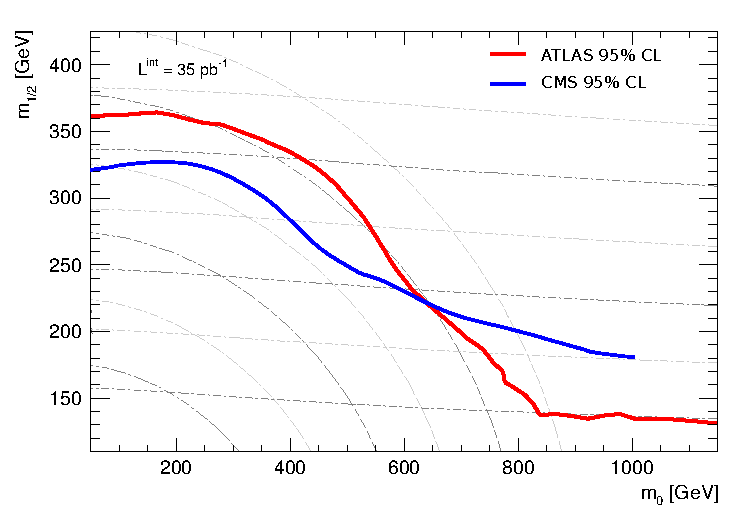
\includegraphics[height=4cm]{atlascms.pdf}
      %\end{tikzpicture}
    \end{column}
  \end{columns}
\end{frame}

\begin{frame}{CMS: SUSY Higgs}
  \begin{columns}
    \begin{column}{0.5\textwidth}
      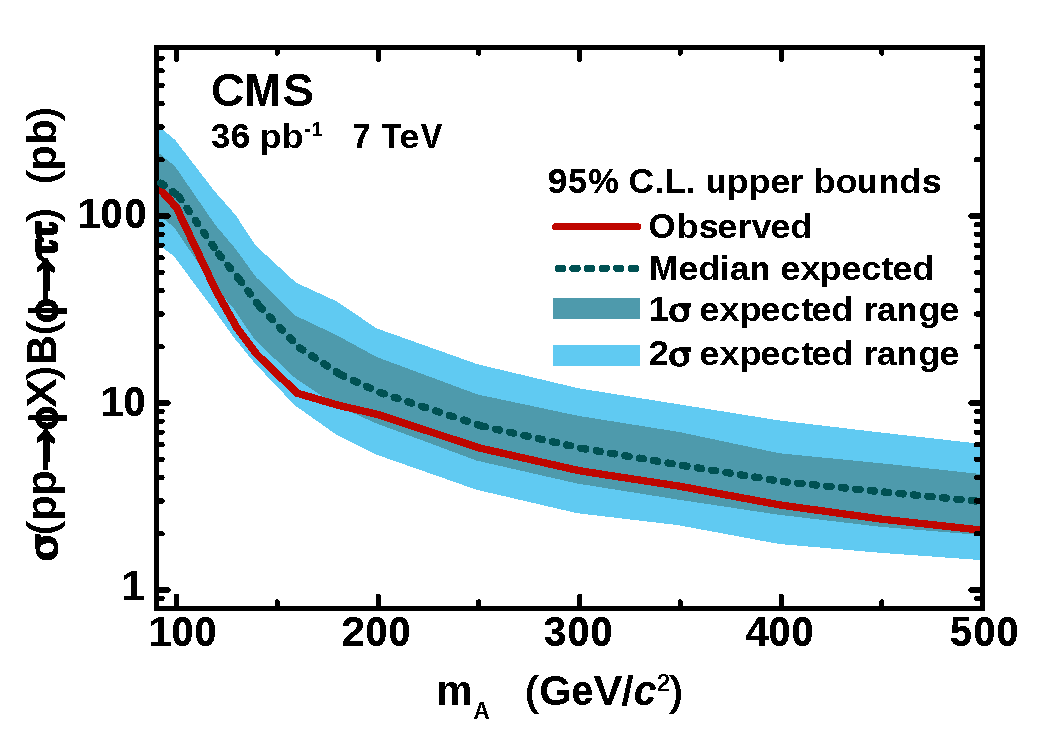
\includegraphics[height=4cm]{htt95.pdf}
      \vfill
    \end{column}

    \begin{column}{0.5\textwidth}
      For fixed values of $M_{A}$ assume
      \begin{equation*}
        \chi^{2}\propto\left(\sigma\times\textrm{BR}\right)^{p\left(M_{A}\right)}
      \end{equation*}
      \begin{itemize}
        \item use the three contours to fit for $p\left(M_{A}\right)$
        \item in the region of interest
        $\left(\sigma\times\textrm{BR}\right)\propto\tan^{2}\left(\beta\right)$
      \end{itemize}
      \begin{equation*}
        \chi^{2}\sim\left(\frac{\tan^{2}\left(\beta\right)}{\tan^{2}\left(\beta\right)_{95\%}}\right)^{p\left(M_{A}\right)}
      \end{equation*}
    \end{column}
  \end{columns}
\end{frame}

\begin{frame}{LHCb, D0 and CDF: $BR(B_{s}\rightarrow\mu\mu)$}
  \begin{columns}
    \begin{column}{0.5\textwidth}
      Combine LHCb (left) with the D0 and CDF
      results
      \begin{itemize}
        \item Use toy experiments to recreate the 90\% CL upper limits from each
        experiment
        \item Toys recreate the 95\% CL limits
        \item Combine using $CL_{s}$ method: generate likelihood
        function.  
      \end{itemize}
    \end{column}
    \begin{column}{0.5\textwidth}
      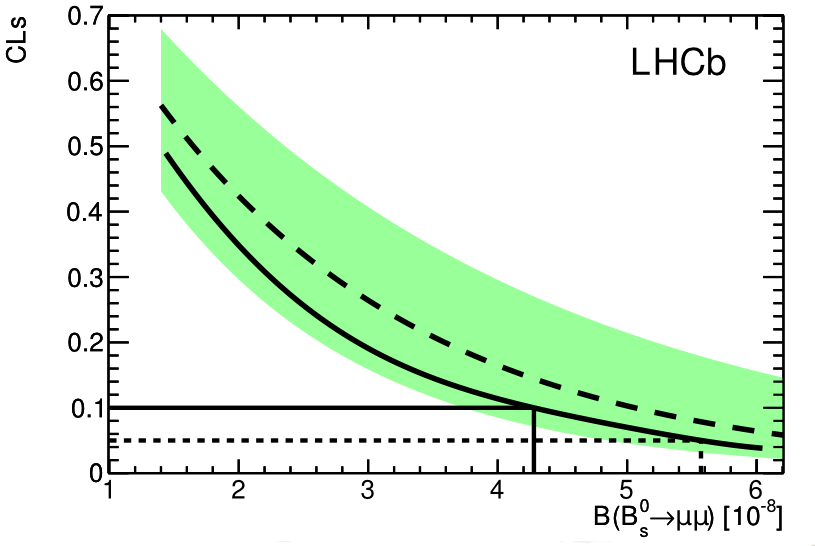
\includegraphics[height=3.4cm]{lhcbBR.png}
    \end{column}
  \end{columns}
  \vfill
  Treat 
  \begin{columns}
    \begin{column}{0.15\textwidth}
      \begin{itemize}
        \item $f_{d}/f_{s}$ 
      \end{itemize}
     \end{column}
    \begin{column}{0.85\textwidth}
      \begin{itemize}
        \item $\textrm{BR}\left(B^{+}\rightarrow
        J/\psi\left(\mu^{+}\mu^{-}\right)K^{+}\right)$
      \end{itemize}
     \end{column}
  \end{columns}
  \vfill
  as common errors
\end{frame}

\begin{frame}{Xenon100}
  \begin{columns}
    \begin{column}{0.55\textwidth}
      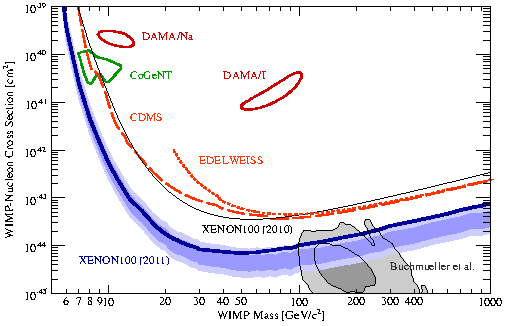
\includegraphics[height=4cm]{xenon.pdf}\\
      The uncertainty on the $\pi$-nucleon $\sigma$ term is also accounted for,
      where we look at both 
      \begin{columns} 
        \begin{column}{0.5\textwidth}
          \begin{itemize}
            \item \small$\Sigma_{\pi N}=50\pm14$
          \end{itemize}
        \end{column}

        \begin{column}{0.5\textwidth}
          \begin{itemize}
            \item \small$\Sigma_{\pi N}=64\pm8$
          \end{itemize}
        \end{column}
      \end{columns}
    \end{column}

    \begin{column}{0.45\textwidth}
      \begin{itemize}
        \item Construct likelihood model for event numbers using $CL_{s}$ method
        \item Close to a Gaussian with $\mu=1.2$, $\sigma=3.2$
        \item 90\% $CL$ corresponds to 6.1 events, rescale from contour (left)
        \item The excess in the Xenon experiments leads to a contribution
        $\chi^{2}\sim0.3$ for small $\sigma_{p}^{SI}$
      \end{itemize}
    \end{column}
  \end{columns}
\end{frame}

\section{Search Impact}
\begin{frame}{Sparticles}
  \begin{columns}
    \begin{column}{0.5\textwidth}
      \rotatebox{90}{\small\textbf{NUHM1}}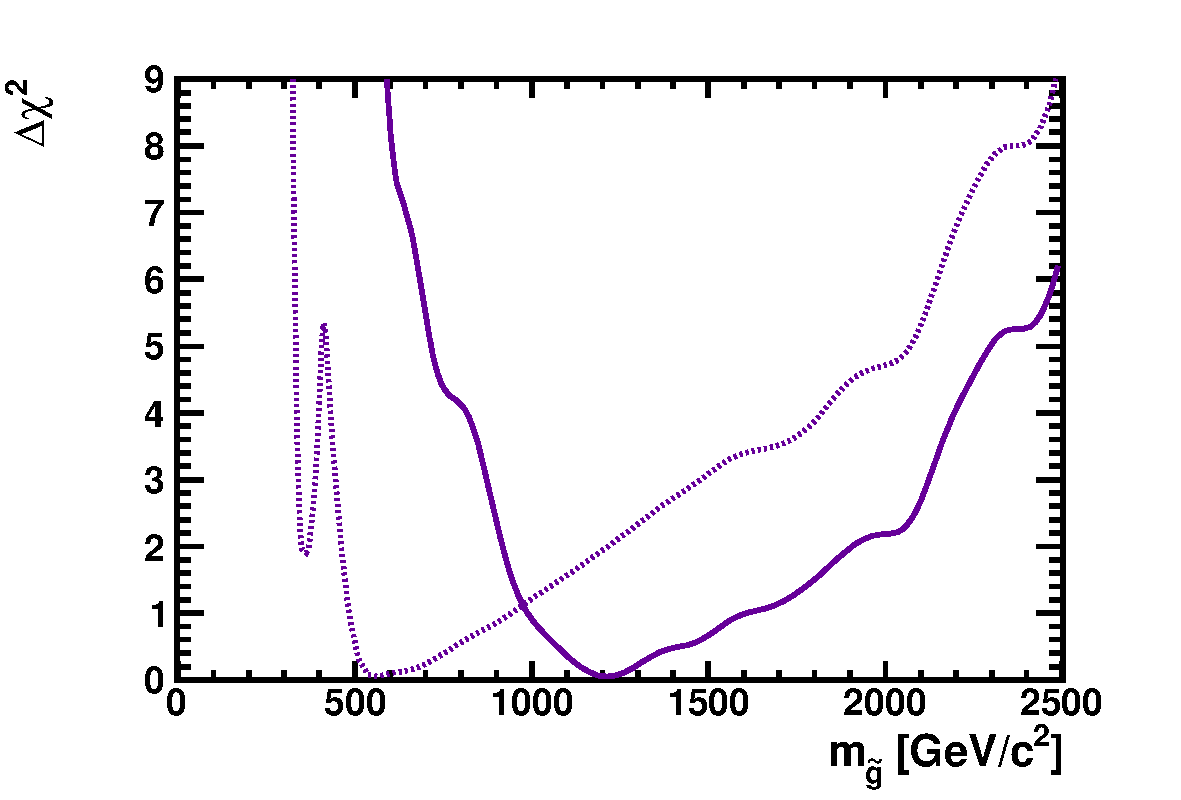
\includegraphics[height=3.2cm]{mg/nuhm1.pdf}\vfill 
      \rotatebox{90}{\small\textbf{CMSSM}}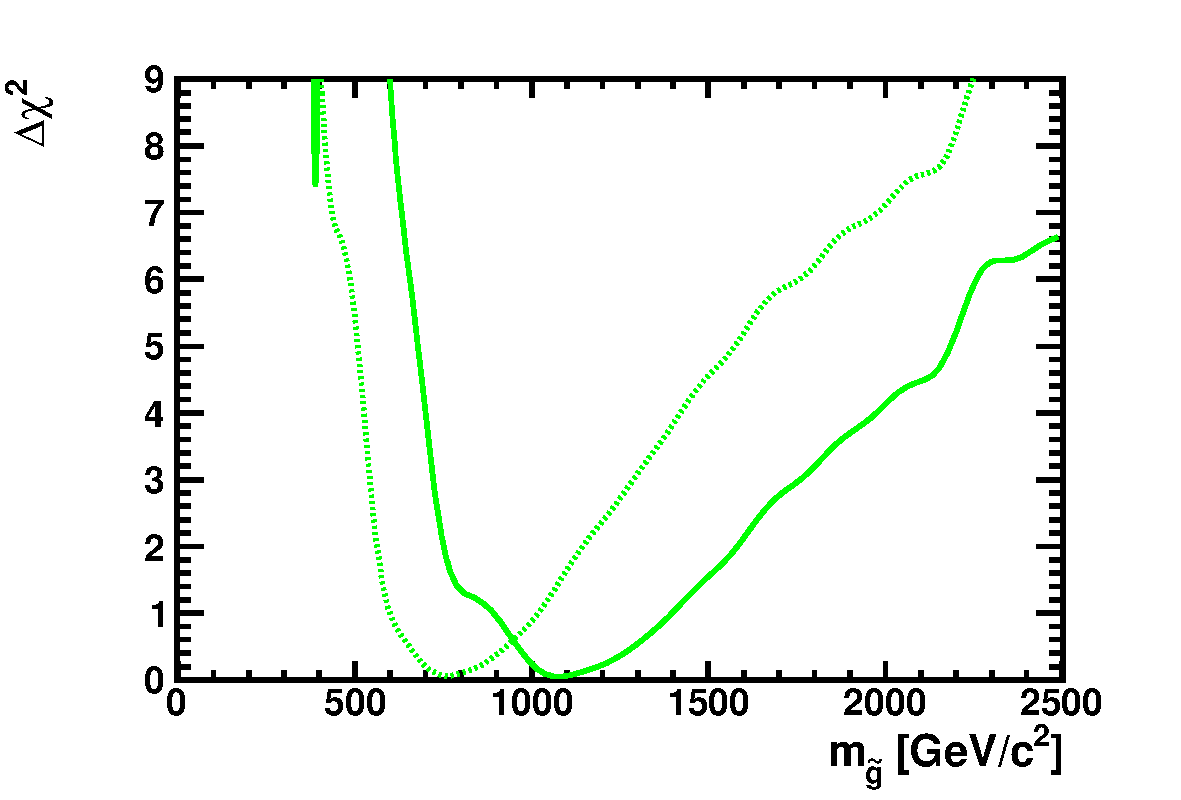
\includegraphics[height=3.2cm]{mg/cmssm.pdf}
    \end{column}
    \begin{column}{0.5\textwidth}
      \rotatebox{90}{\small\textbf{VCMSSM}}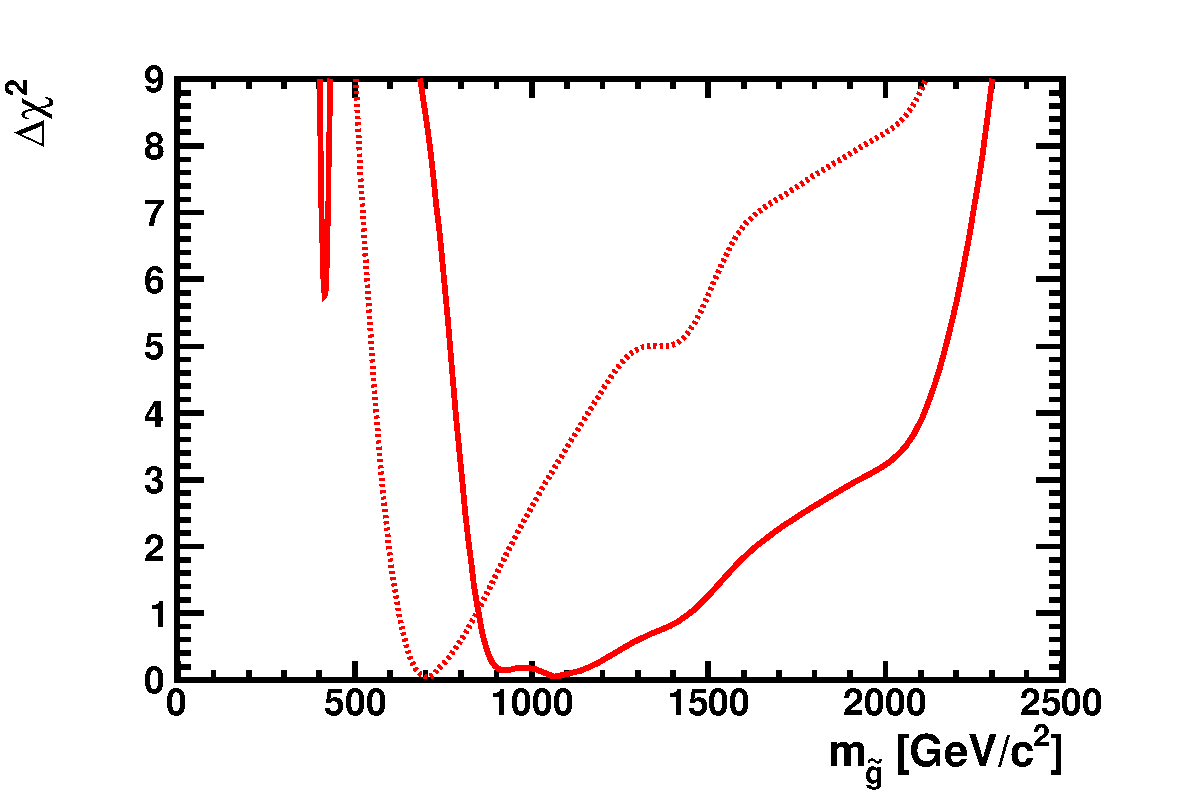
\includegraphics[height=3.2cm]{mg/vcmssm.pdf}\vfill 
      \rotatebox{90}{\small\textbf{mSUGRA}}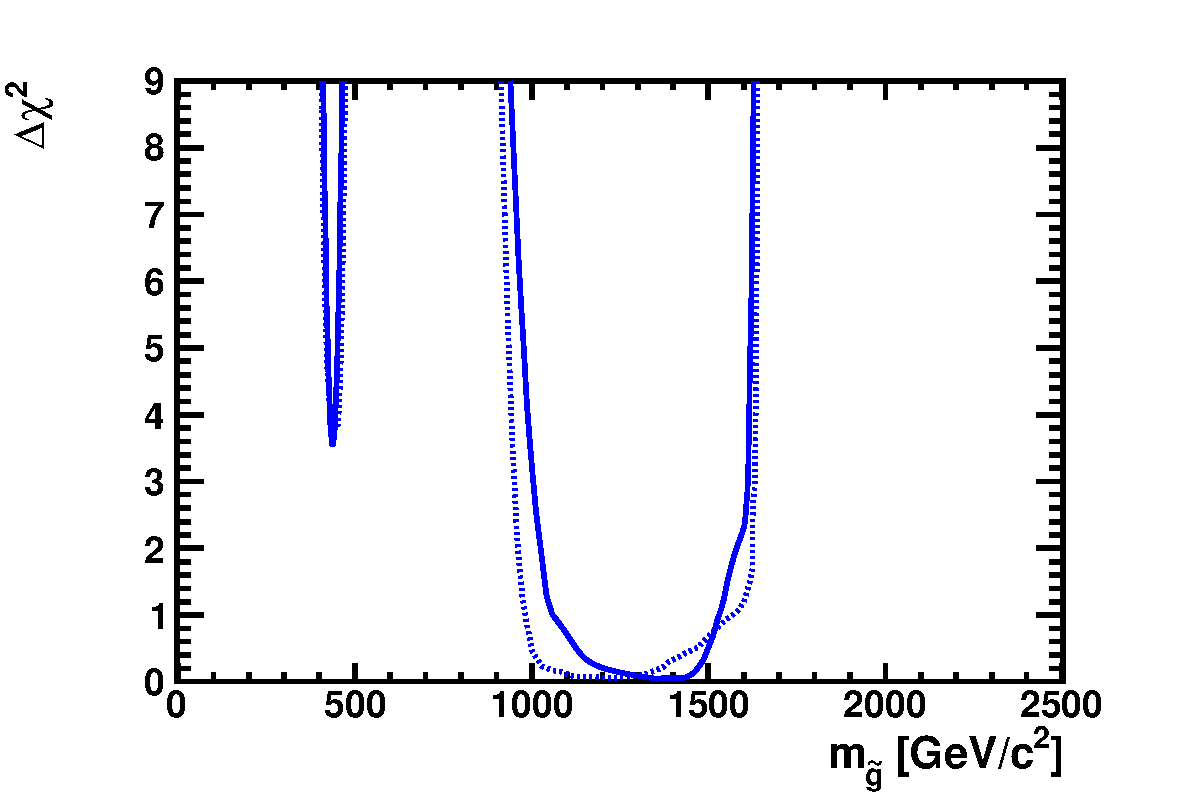
\includegraphics[height=3.2cm]{mg/msugra.pdf}
    \end{column}
  \end{columns}
\end{frame}

\begin{frame}{Lightest MSSM Higgs mass}
  \begin{columns}
    \begin{column}{0.5\textwidth}
      \rotatebox{90}{\small\textbf{NUHM1}}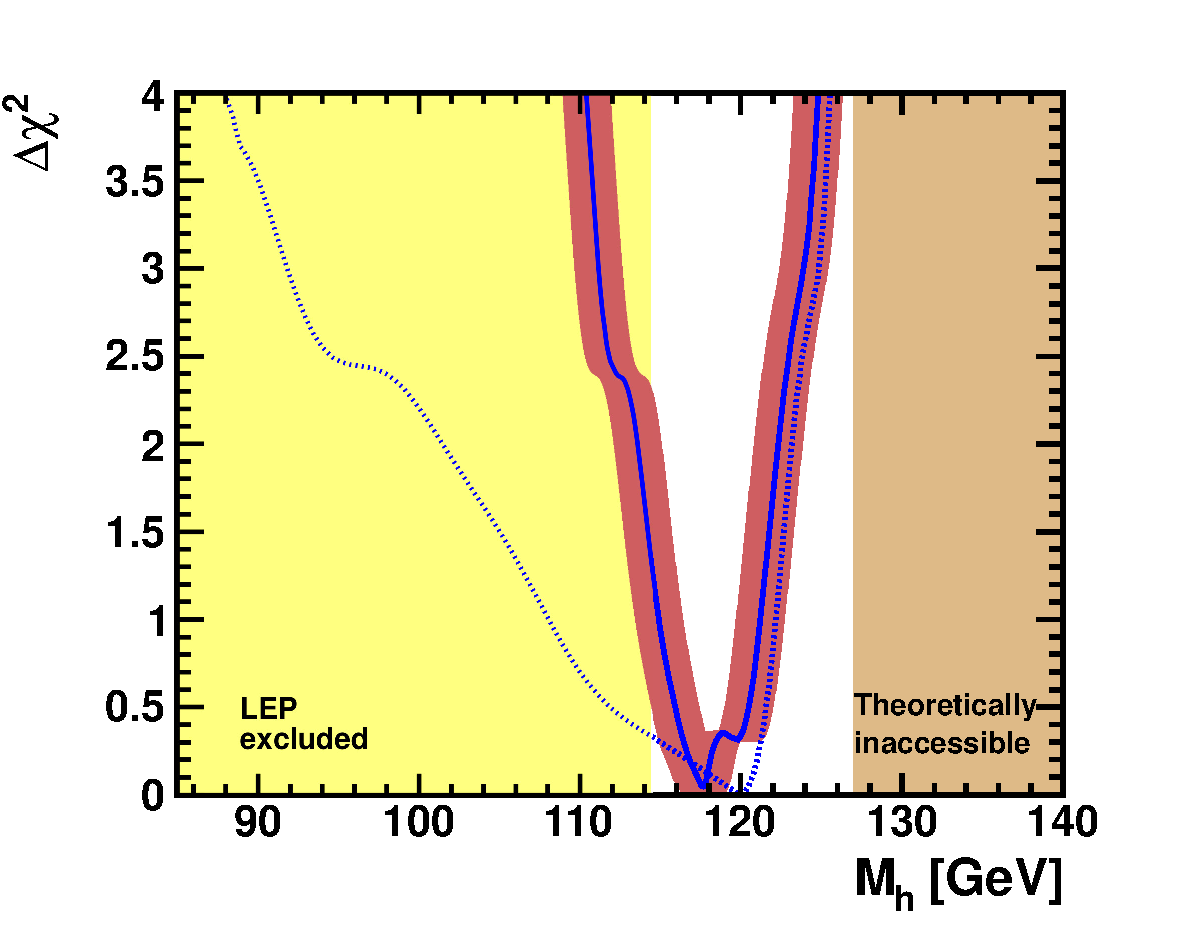
\includegraphics[height=3.3cm]{mh/nuhm1.pdf}\vfill 
      \rotatebox{90}{\small\textbf{\ CMSSM}}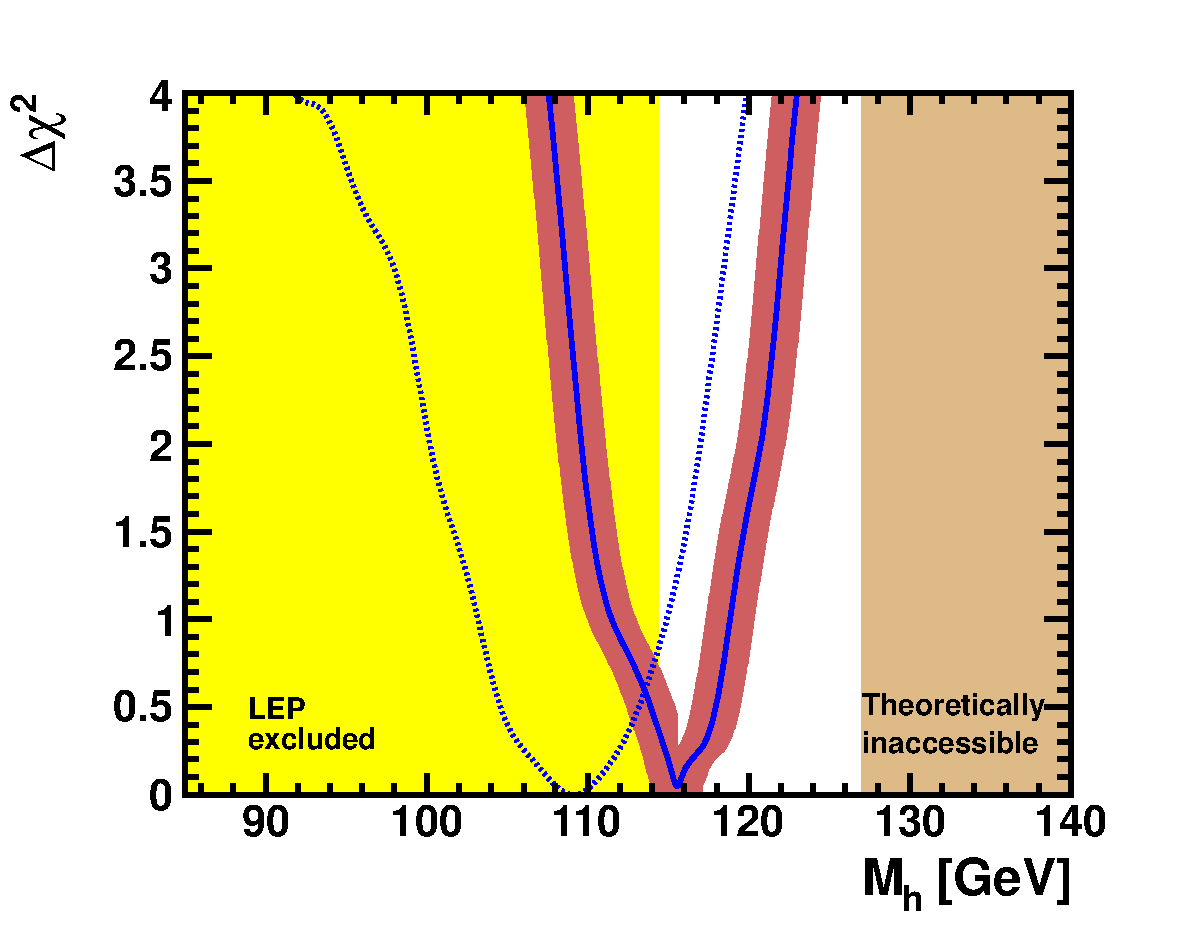
\includegraphics[height=3.3cm]{mh/cmssm.pdf}
    \end{column}
    \begin{column}{0.5\textwidth}
      \rotatebox{90}{\small\textbf{VCMSSM}}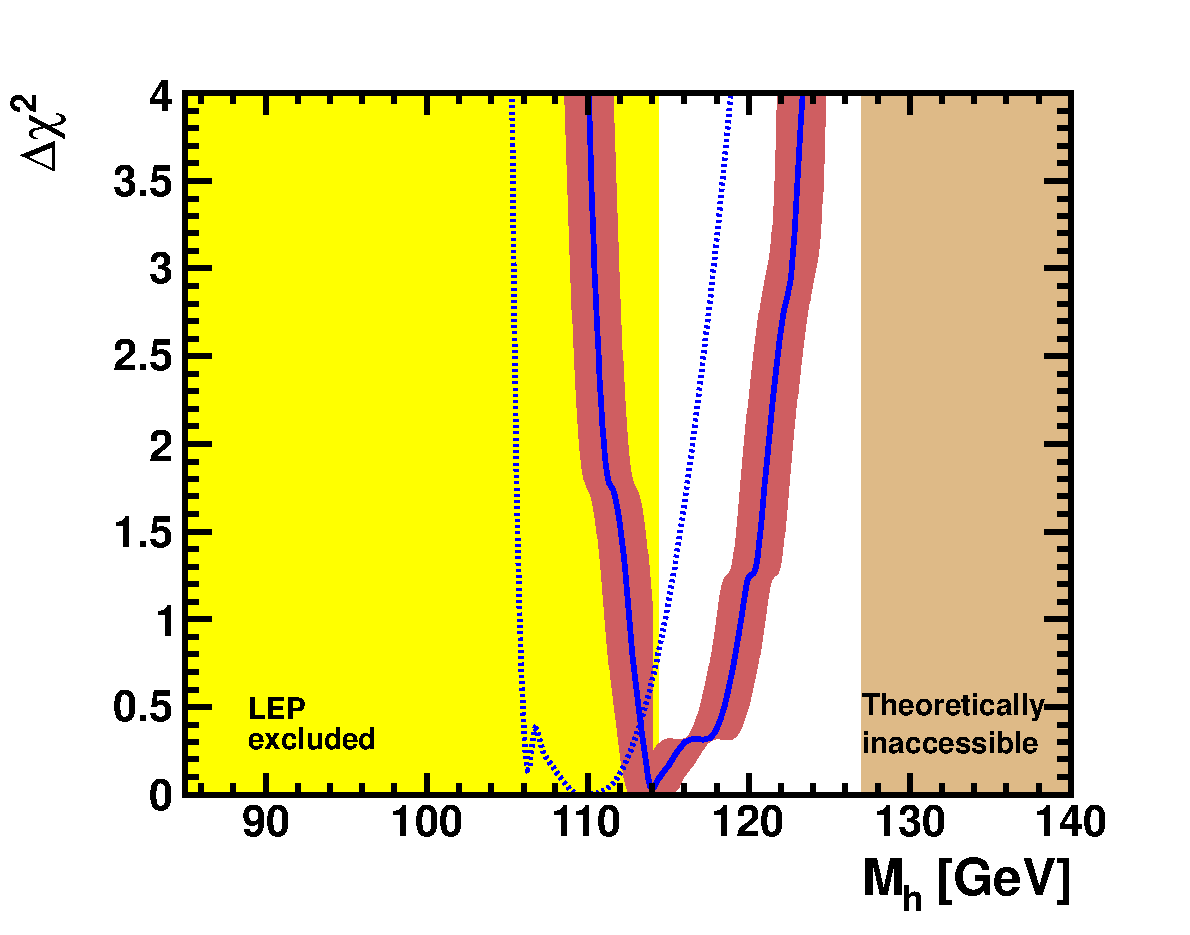
\includegraphics[height=3.3cm]{mh/vcmssm.pdf}\vfill 
      \rotatebox{90}{\small\textbf{\ mSUGRA}}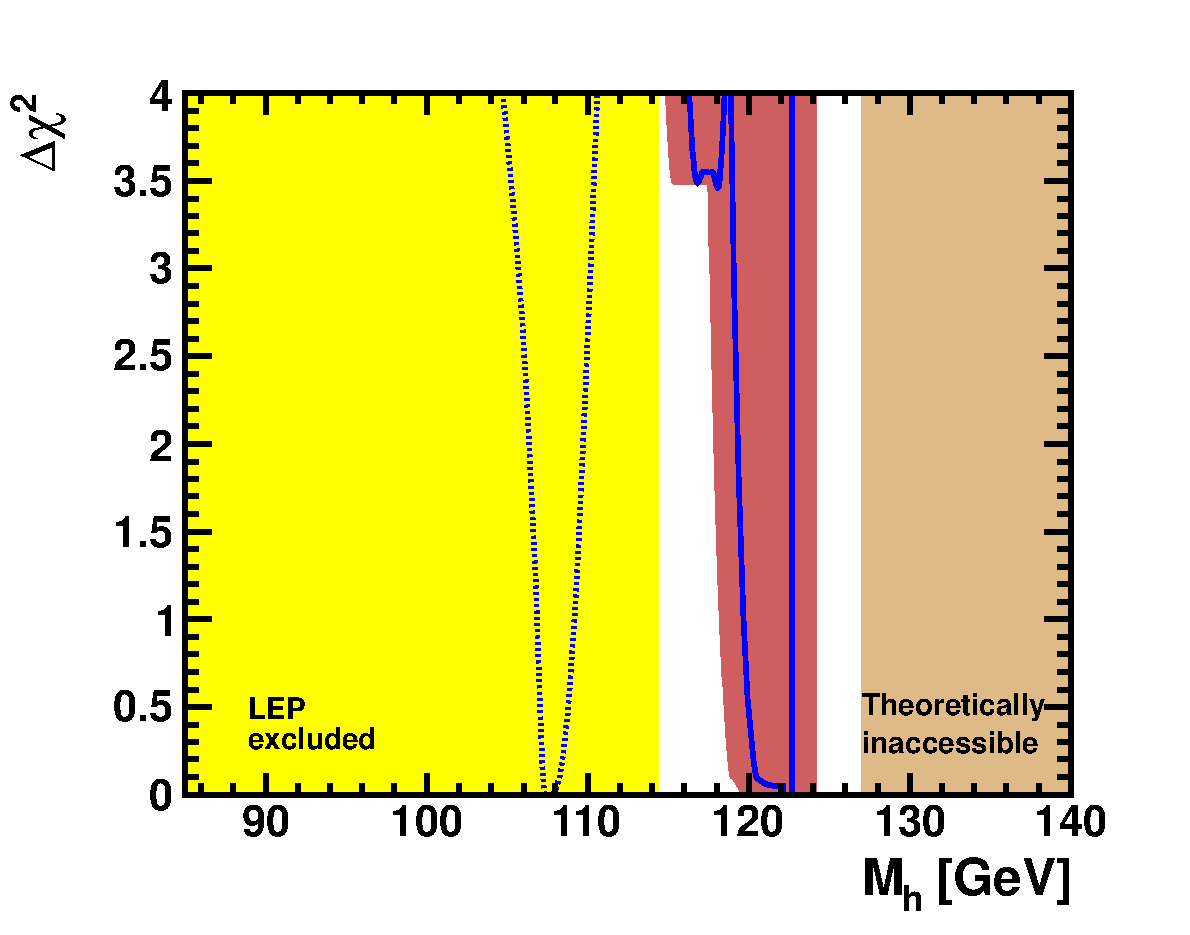
\includegraphics[height=3.3cm]{mh/msugra.pdf}
    \end{column}
  \end{columns}
\end{frame}

\begin{frame}{$\textrm{BR}(B_{s}\rightarrow\mu\mu)$}
  \begin{columns}
    \begin{column}{0.5\textwidth}
      \rotatebox{90}{\small\textbf{NUHM1}}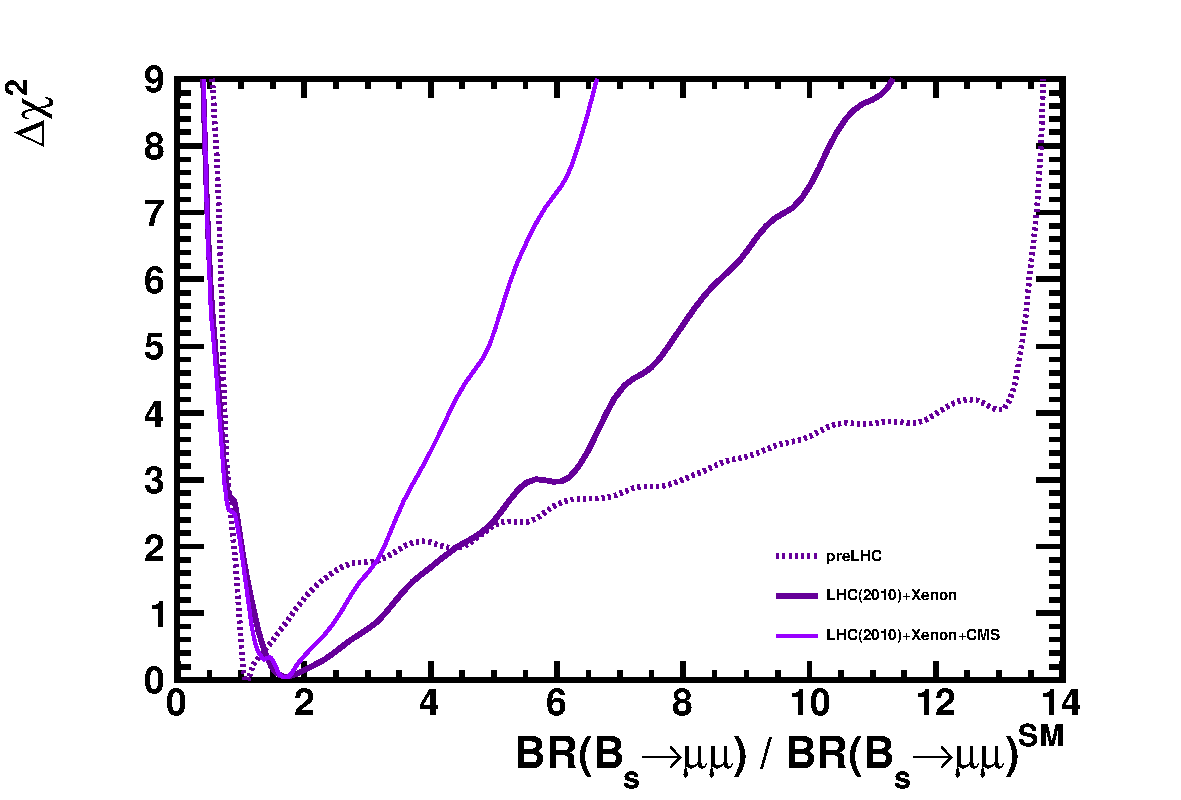
\includegraphics[height=3.2cm]{bsmm/nuhm1.pdf}\vfill 
      \rotatebox{90}{\small\textbf{CMSSM}}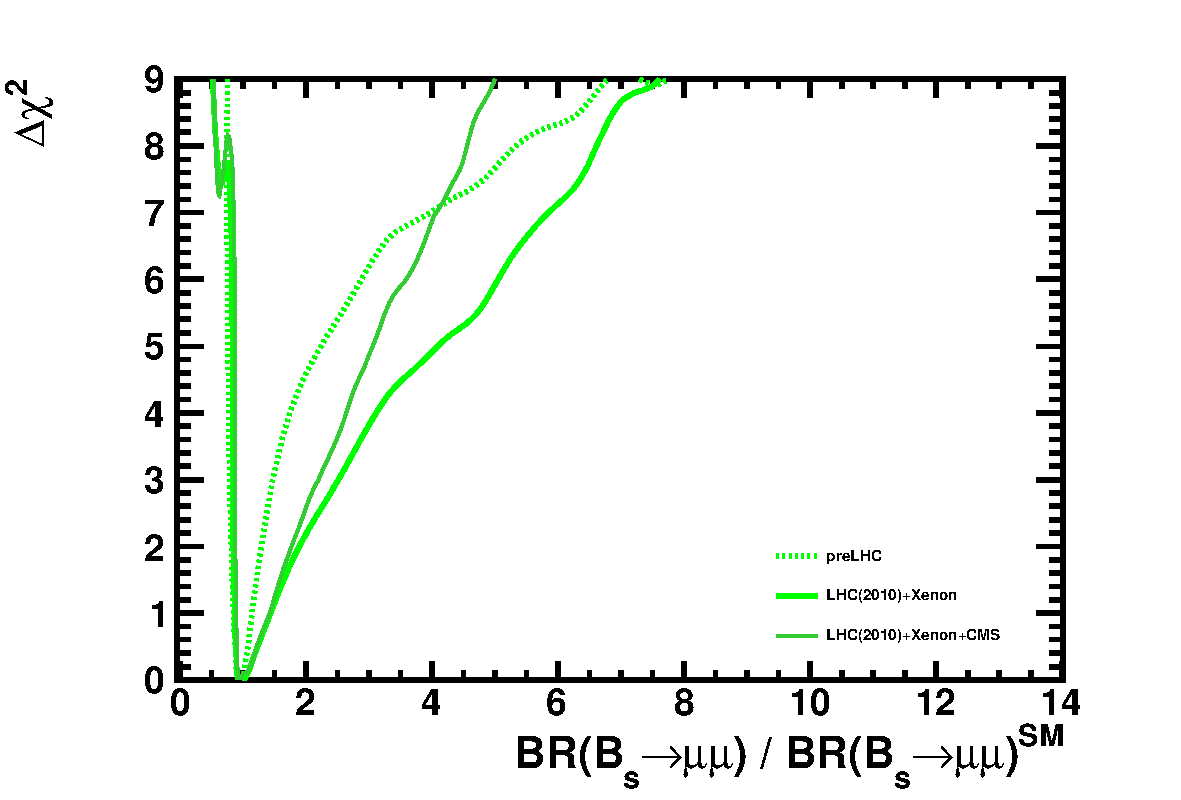
\includegraphics[height=3.2cm]{bsmm/cmssm.pdf}
    \end{column}
    \begin{column}{0.5\textwidth}
      \rotatebox{90}{\small\textbf{VCMSSM}}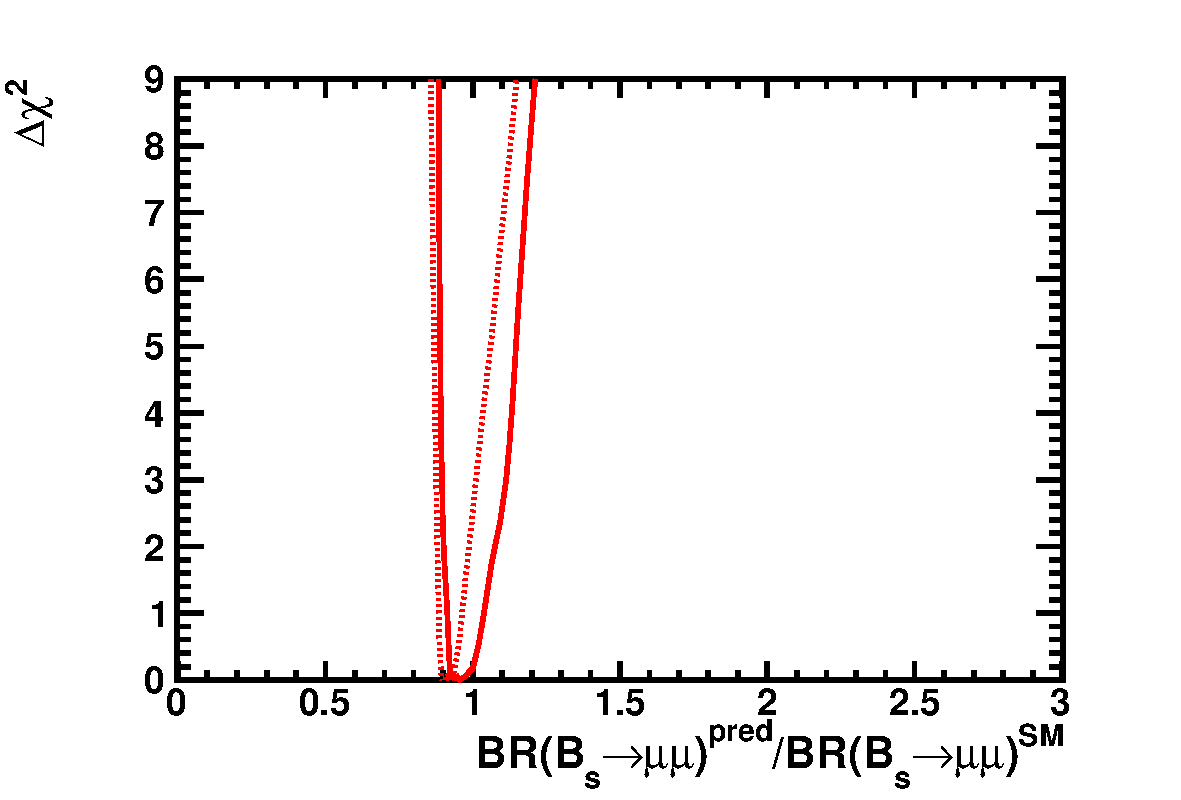
\includegraphics[height=3.2cm]{bsmm/vcmssm.pdf}\vfill 
      \rotatebox{90}{\small\textbf{mSUGRA}}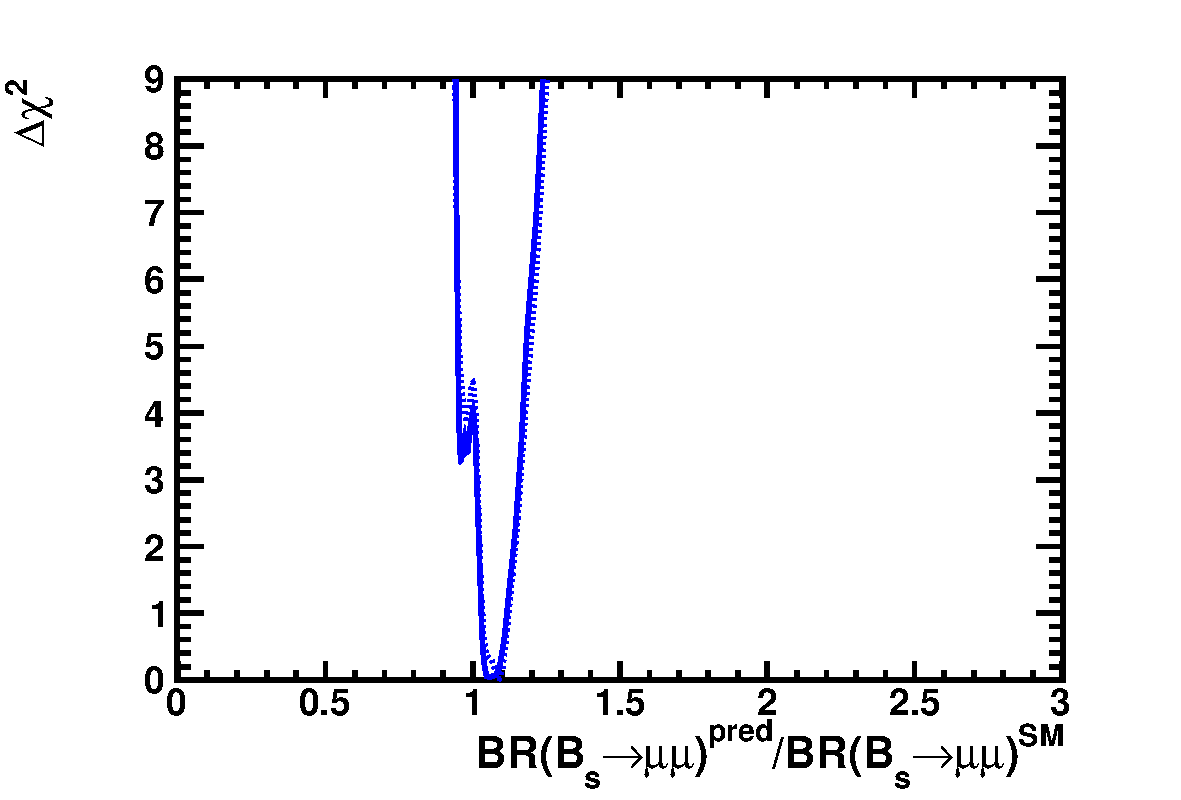
\includegraphics[height=3.2cm]{bsmm/msugra.pdf}
    \end{column}
  \end{columns}
\end{frame}

\begin{frame}{Dark Matter: $\sigma_{p}^{SI}$}
  \begin{columns}
    \begin{column}{0.5\textwidth}
      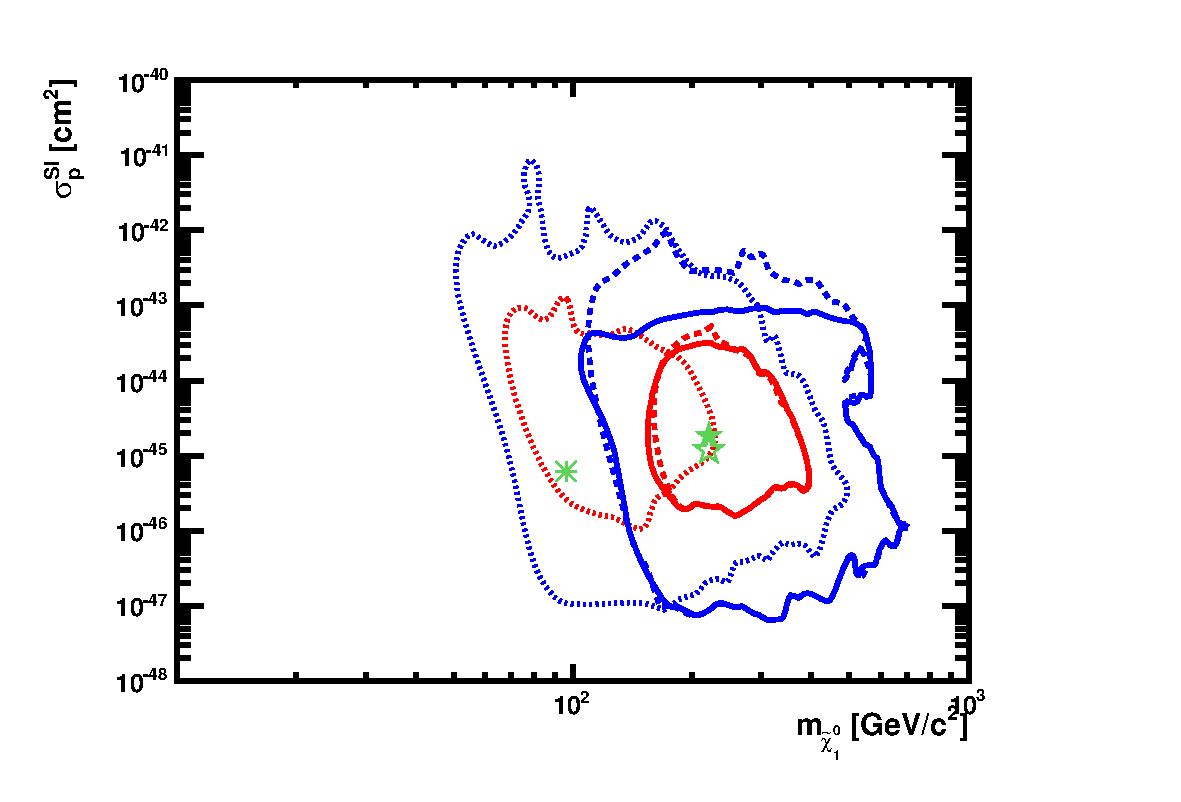
\includegraphics[height=4.5cm]{ssd/nuhm1.pdf}\\ 
      \textbf{NUHM1}
    \end{column}
    \begin{column}{0.5\textwidth}
      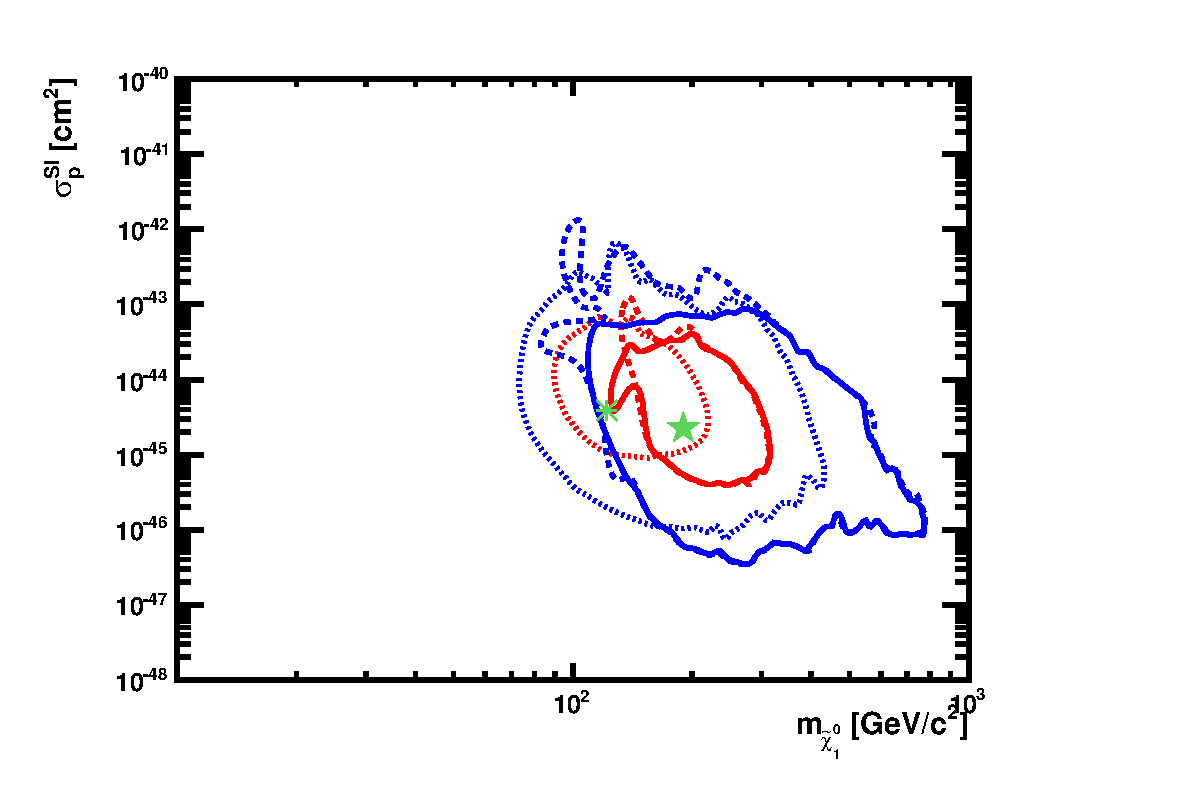
\includegraphics[height=4.5cm]{ssd/cmssm.pdf}\\
      \textbf{CMSSM}
    \end{column}
  \end{columns}
\end{frame}

\begin{frame}{Dark Matter: $\sigma_{p}^{SI}$}
  \begin{columns}
    \begin{column}{0.5\textwidth}
      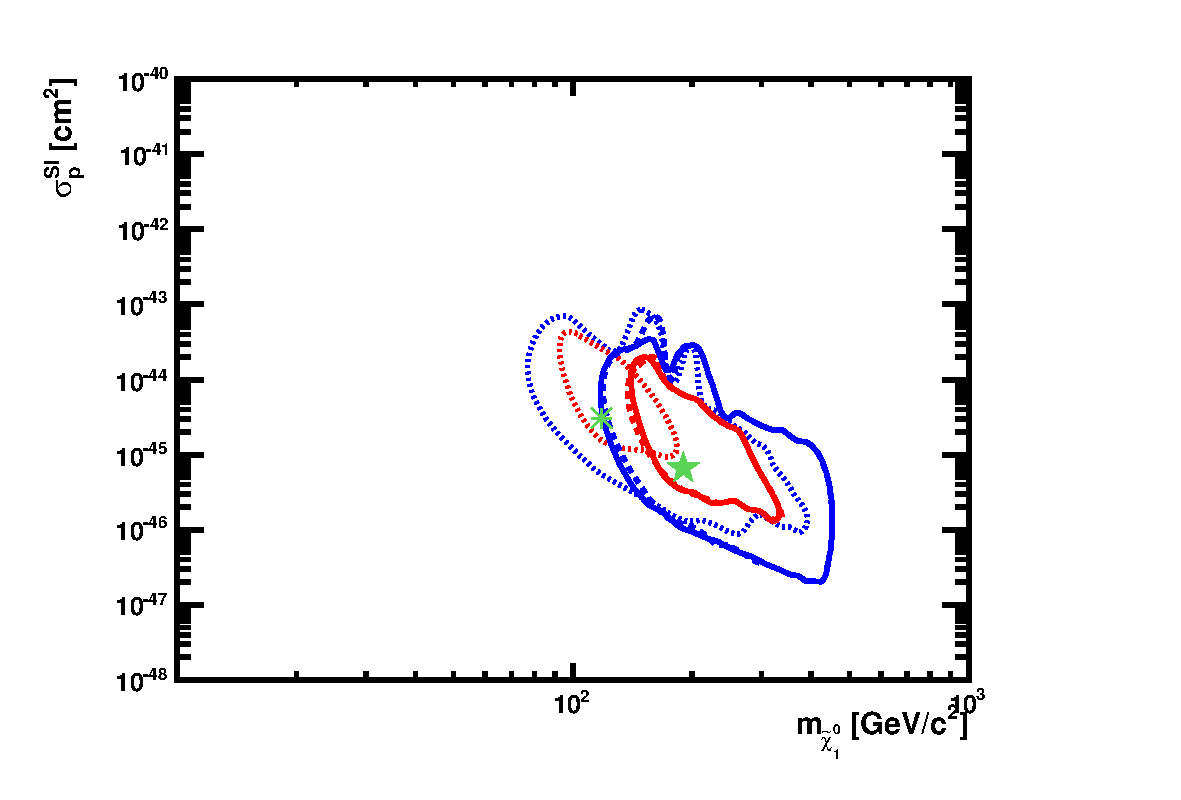
\includegraphics[height=4.5cm]{ssd/vcmssm.pdf}\\ 
      \textbf{VCMSSM}
    \end{column}
    \begin{column}{0.5\textwidth}
      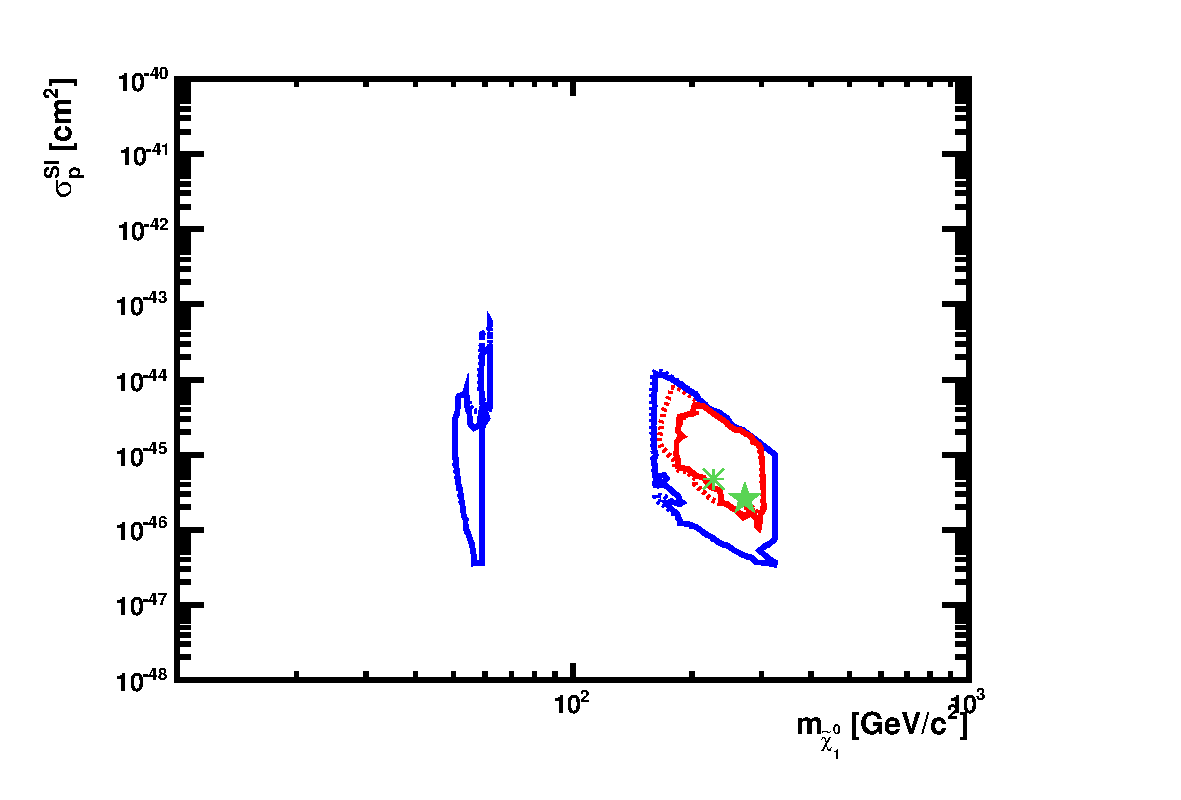
\includegraphics[height=4.5cm]{ssd/msugra.pdf}\\
      \textbf{mSUGRA}
    \end{column}
  \end{columns}
\end{frame}

\section{The Future}
\begin{frame}{Parameter Spaces}
  \begin{columns}
    \begin{column}{0.5\textwidth}
      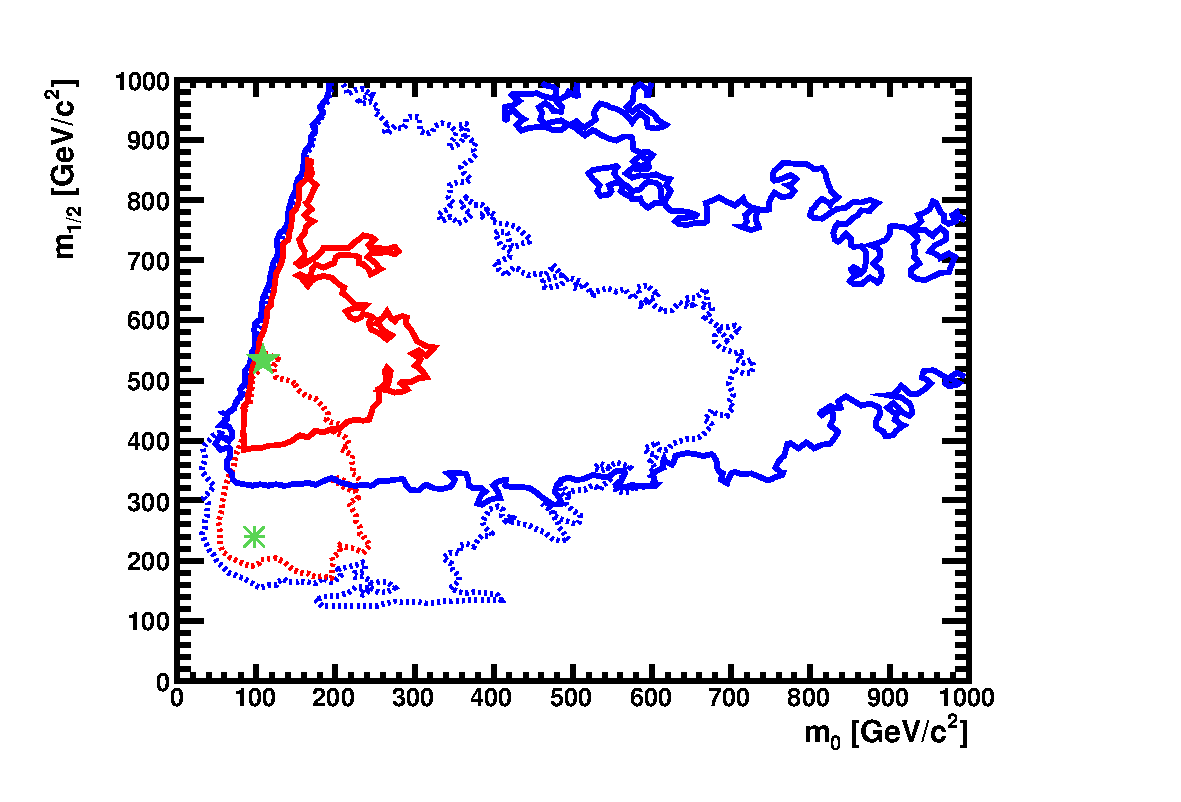
\includegraphics[height=4.5cm]{m0m12/nuhm1.pdf}\\
      \textbf{NUHM1}
    \end{column}
    \begin{column}{0.5\textwidth}
      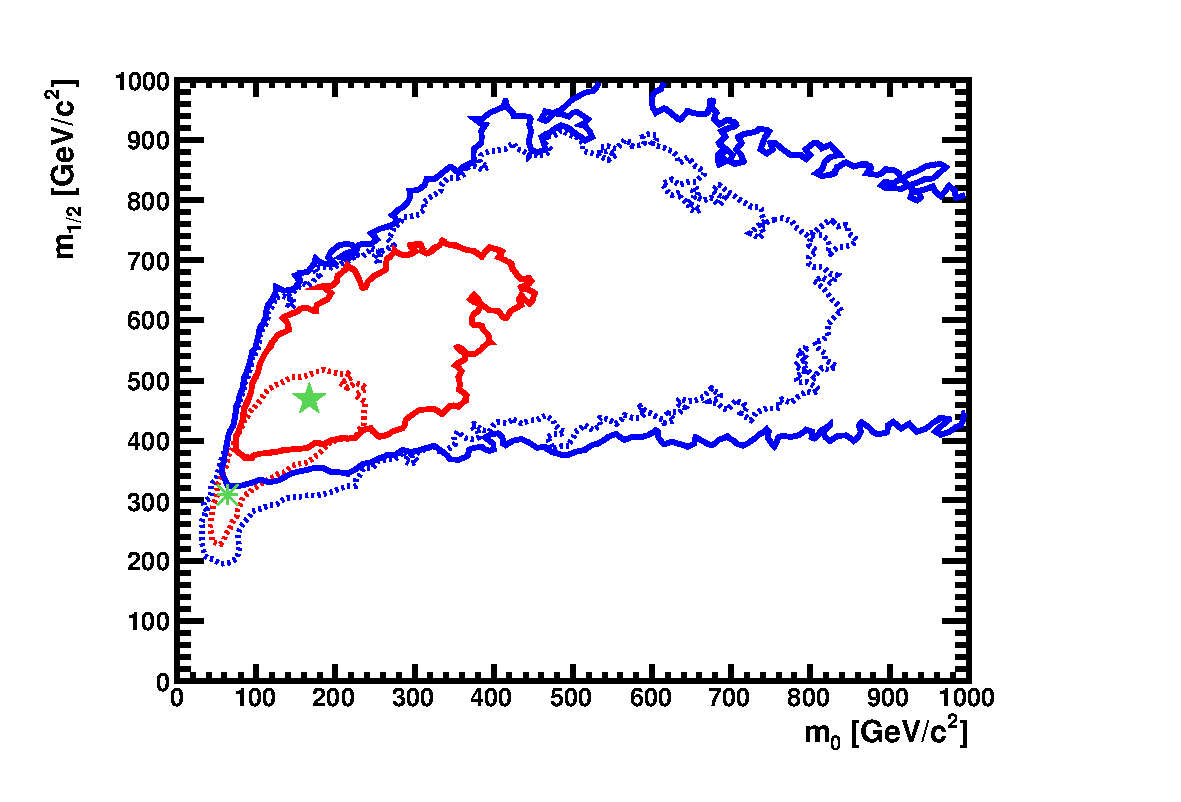
\includegraphics[height=4.5cm]{m0m12/cmssm.pdf}\\
      \textbf{CMSSM}
    \end{column}
  \end{columns}
\end{frame}

\begin{frame}{Parameter Spaces}
  \begin{columns}
    \begin{column}{0.5\textwidth}
      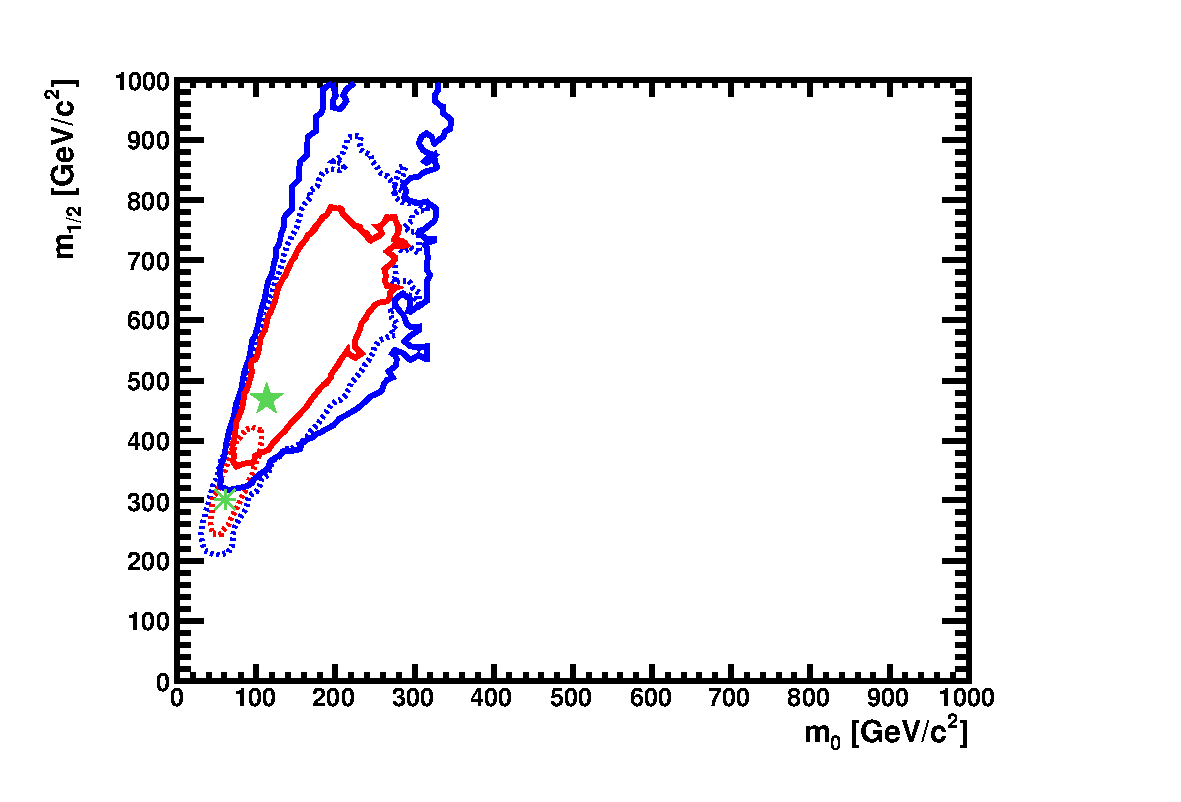
\includegraphics[height=4.5cm]{m0m12/vcmssm.pdf}\\
      \textbf{VCMSSM}
    \end{column}
    \begin{column}{0.5\textwidth}
      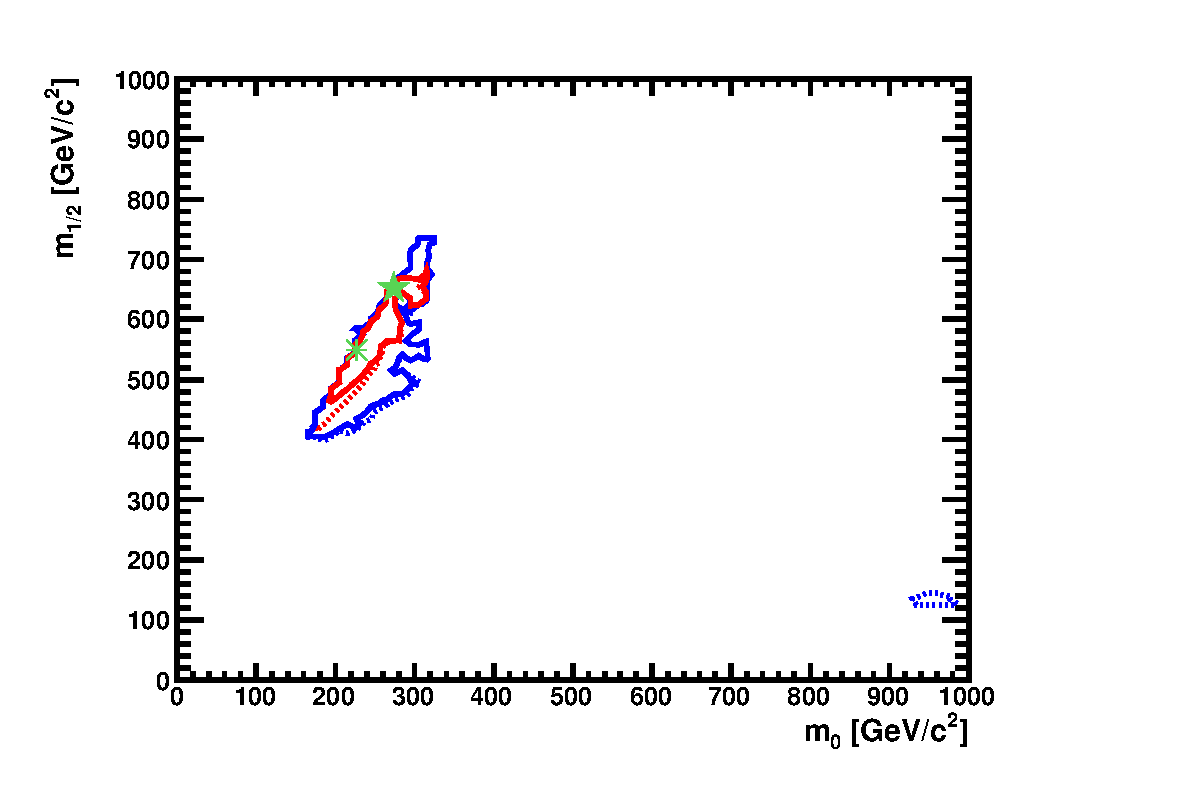
\includegraphics[height=4.5cm]{m0m12/msugra.pdf}\\
      \textbf{mSUGRA}
    \end{column}
  \end{columns}
\end{frame}

\begin{frame}{Model Probabilities}
  \begin{columns}
    \begin{column}{0.5\textwidth}
      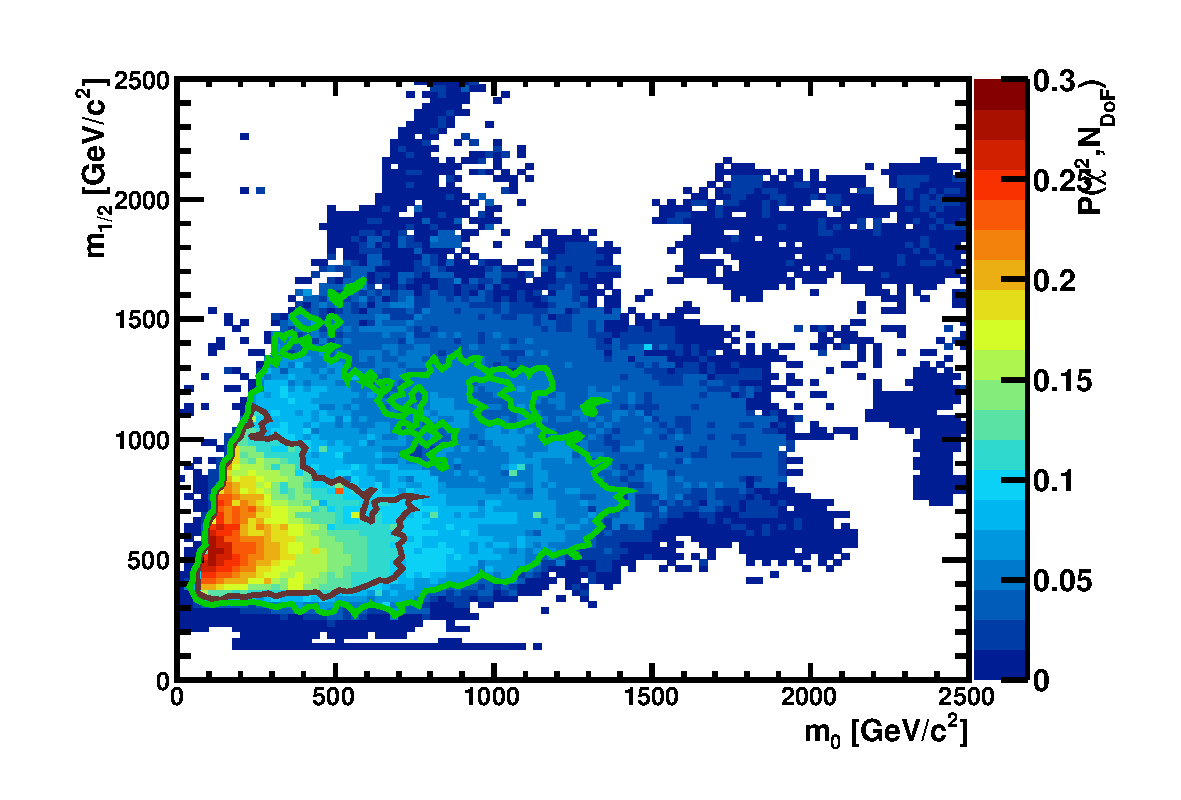
\includegraphics[height=4.3cm]{prob-2010/nuhm1.pdf}\\
      \textbf{NUHM1}
    \end{column}
    \begin{column}{0.5\textwidth}
      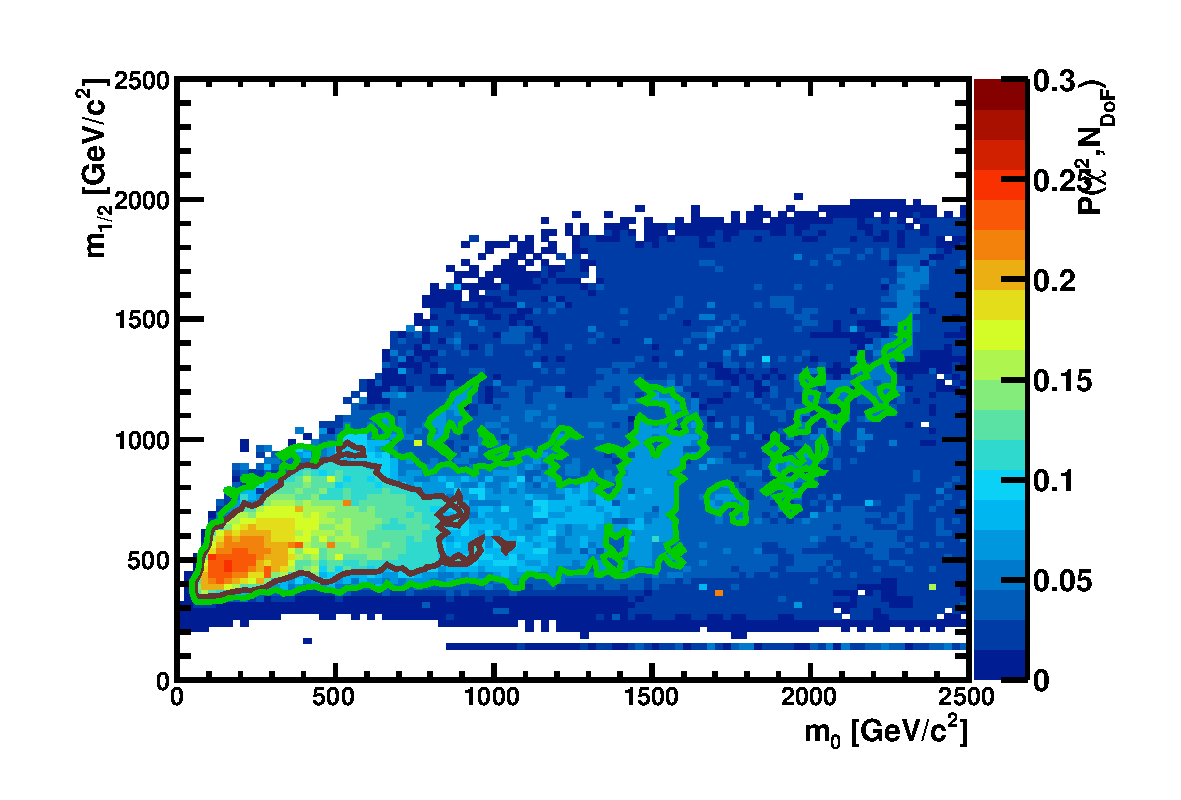
\includegraphics[height=4.3cm]{prob-2010/cmssm.pdf}\\
      \textbf{CMSSM}
    \end{column}
  \end{columns}
  \setlength{\tabcolsep}{5pt}
  \begin{center}
    \tiny
    \begin{tabular}{|r||c|c|c|c|c|c||c|}
      \hline
      Model & Min $\chi^{2}$ & Prob & $m_{1/2}$ & $m_{0}$ & $A_{0}$ &
      $\tan\left(\beta\right)$ & $M_{h}^{\textrm{no LEP}}$  \\
      \hline\hline
      \alert{CMSSM} & 22.5/19 & 26\% & 310 & 60 & -60 & 10 & 109 \\
       post-LHC/Xenon & 26.2/20 & 16\% & 470 & 170 & -780 & 22 & 116 \\
      \hline  
      \alert{NUHM1} & 20.5/17 & 25\% & 240 & 100 & 920 & 7 & 119 \\
       post-LHC/Xenon & 24.2/19 & 19\% & 530 & 110 & -370 & 27 & 118 \\
      \hline
     
    \end{tabular}
  \end{center}
\end{frame}

\begin{frame}{Summary}
  \begin{itemize}
    \item $m_{\tilde{g}}> 1\textrm{TeV}$
    \item $m_{h^{0}}>115\textrm{GeV}$
    \item $\textrm{BR}\left(B_{s}\rightarrow\mu\mu\right)$ preferred at
    $\sim1\times\textrm{SM}$: CMS 1.9e-8 ($5.5\times\textrm{SM}$@95\%)
    \item $P\left(\chi^{2},n_{D}\right)_{\textrm{model}}$ falling.
    $P\sim0.1$.  $1fb^{-1}$ searches: expect to see $P<0.05$.
    \item \emph{Air is starting to become very thin for these constrained models of
    SUSY}
  \end{itemize}
\end{frame}

\begin{frame}{BACKUP SLIDES}
\end{frame}

\begin{frame}{Thresholds}
      %\begin{tikzpicture}[remember picture,overlay]  
      %    \node [xshift=-2cm,yshift=-2cm] at (current page.north east)
            \hfill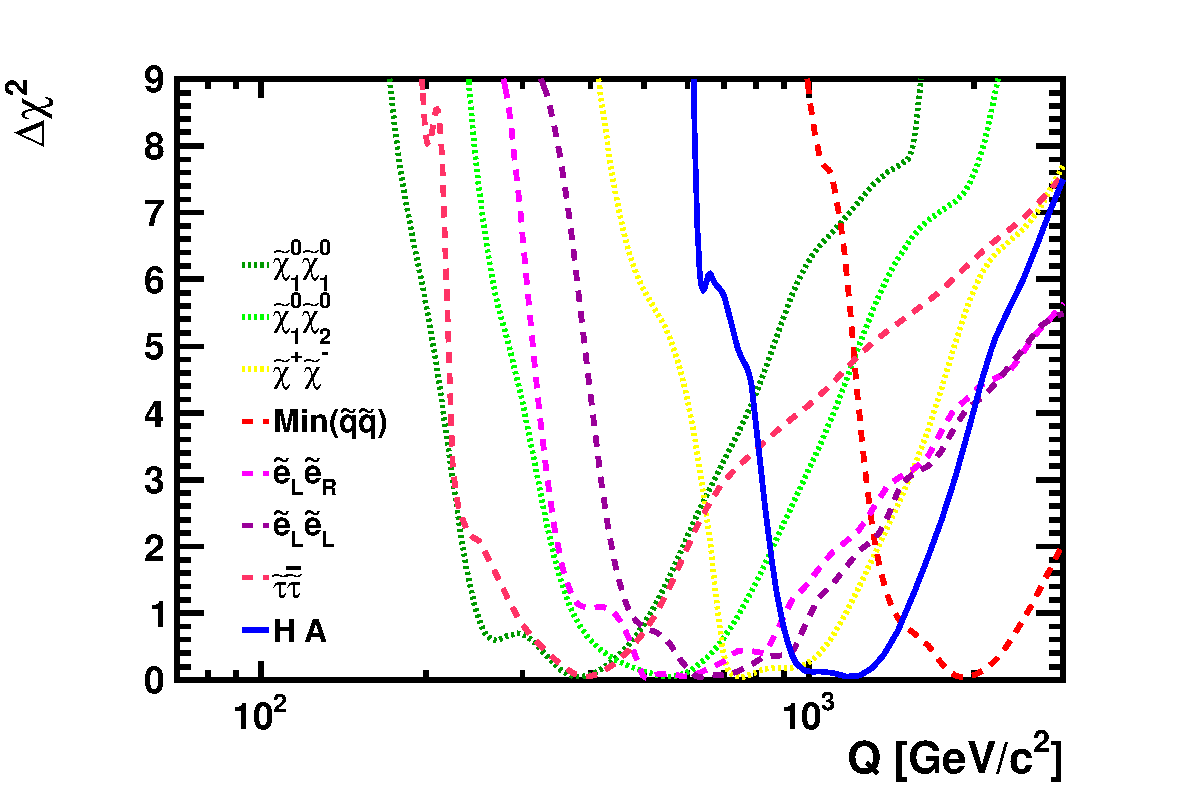
\includegraphics[height=4cm]{thresh/cmssm.pdf}
      %\end{tikzpicture}
      %\begin{tikzpicture}[remember picture,overlay]  
      %    \node [xshift=-2cm,yshift=-2cm] at (current page.north east)
            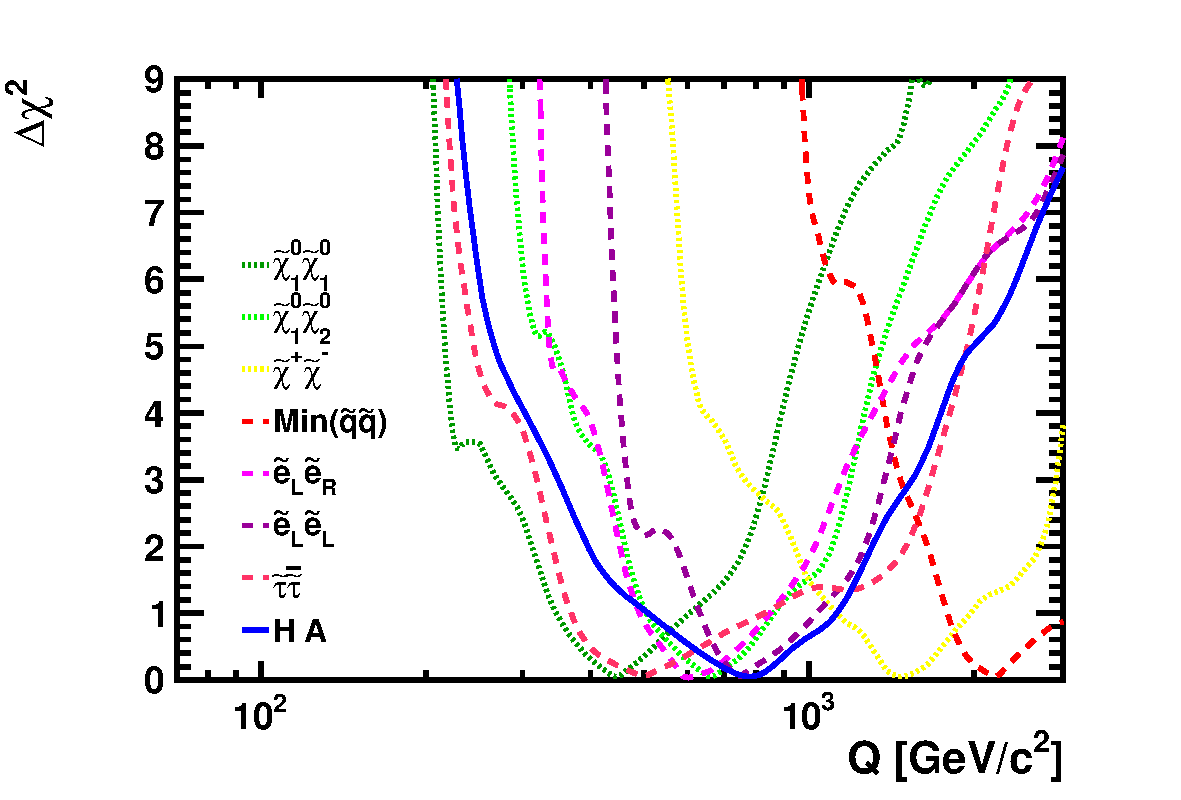
\includegraphics[height=4cm]{thresh/nuhm1.pdf}\hfill
      %\end{tikzpicture}
\end{frame}


\end{document}
